% Based on:
% https://www.overleaf.com/learn/latex/Posters
\documentclass[25pt]{tikzposter}
\geometry{paperwidth=36in,paperheight=42in}
\usepackage[utf8]{inputenc}

\usepackage{adjustbox}
\usepackage{ragged2e}

\usepackage{svg}
\usetikzlibrary{shapes,arrows,positioning}

\usepackage[
backend=biber,
style=numeric,
]{biblatex}
\addbibresource{refs.bib}

\newcommand{\imgh}{7em}
\newcommand{\sampleimgh}{10em}

\title{Image Vectorization for Architecture}
\author{Jonathan Lam, Derek Lee, Victor Zhang}
\institute{Prof. Samuel Keene \\ \vspace{16pt} The Cooper Union for the Advancement of Science and Art}

\usetheme{Simple}

\begin{document}

\maketitle

\block{Abstract}{
  {\fontsize{40}{48}\selectfont Vector (shape-based) images are a useful image representation that may be more efficient than traditional raster (pixel-besed) formats. Our project aims to develop a image vectorization method (a tool to convert from raster to vector format) specialized towards architecture images (or other highly-geometric images), and explores the potential of vector-based images in the architecture design process and as machine learning preprocessing.}
}

\block{Algorithm/Architecture}{
  {\fontsize{40}{48}\selectfont A raster image is first sampled using blue noise sampling (BNS) \cite{zhao2013image}, which generates a point cloud with variable density. This point cloud is simplified using the quadric error metric (QEM) \cite{hoppe1999new}. We also run the image through multiple color scans using the Potrace edge tracing algorithm \cite{selinger2003potrace}. Then the point cloud is vectorized using a triangulation method and the edges are improved using the Potrace scans, and is outputted to a SVG format. We evaluate the accuracy of the generated image using content loss \cite{dumoulin2017learned}.}

  \vspace{48pt}

  \begin{center}
    \begin{tikzpicture}[picBlock/.style = {rectangle, draw, fill=white, text width=10em,
        text centered, rounded corners, minimum size=7.5em},
      textBlock/.style = {rectangle, fill=white, text width=10em,
        text centered, rounded corners, minimum height=2em},
      node distance=4cm]
      \node[] (original) {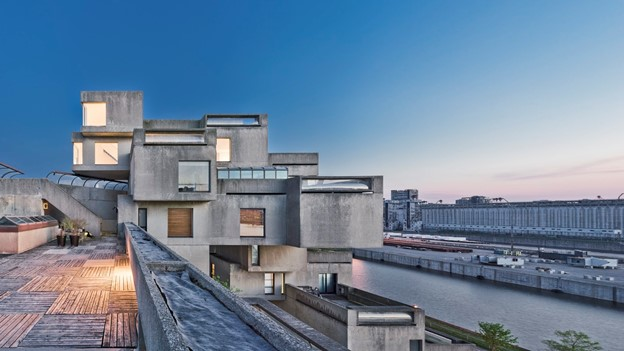
\includegraphics[height=\imgh]{Figures/house.jpg}};
      \node[textBlock, below=0.25cm of original] {Original image};

      \node[above right=-1cm and 5cm of original] (importance) {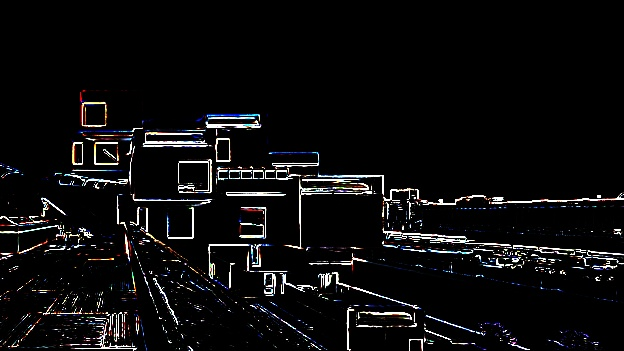
\includegraphics[height=\imgh]{Figures/Arch_Diagram/importance.jpg}};
      \node[textBlock, below=0.25cm of importance] (importance_label) {Importance sampling};

      \node[right=of importance] (sampling) {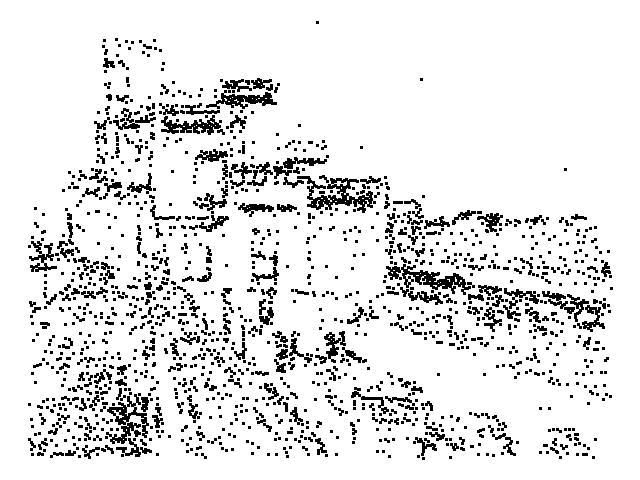
\includegraphics[height=\imgh]{Figures/Arch_Diagram/sampled.jpg}};
      \node[textBlock, below=0.25cm of sampling] {Sampled points};

      \node[right=of sampling] (decimation) {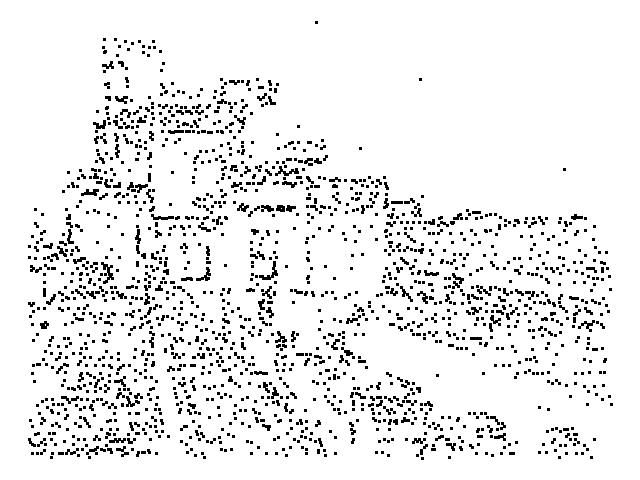
\includegraphics[height=\imgh]{Figures/Arch_Diagram/decimated.jpg}};
      \node[textBlock, below=0.25cm of decimation] {Decimated points};

      \node[right=of decimation] (triangulation) {\includesvg[height=\imgh]{Figures/house.svg}};
      \node[textBlock, below=0.25cm of triangulation] {Triangulated image};

      \node[below right=-1cm and 5cm of original] (potrace_scan1) {\includesvg[height=\imgh]{Figures/Arch_Diagram/scan0.svg}};
      \node[below right=0.5cm and 0.5cm of potrace_scan1.north west] (potrace_scan2) {\includesvg[height=\imgh]{Figures/Arch_Diagram/scan1.svg}};
      \node[below right=1.0cm and 1.0cm of potrace_scan1.north west] (potrace_scan3) {\includesvg[height=\imgh]{Figures/Arch_Diagram/scan2.svg}};
      \node[below right=1.5cm and 1.5cm of potrace_scan1.north west] (potrace_scan4) {\includesvg[height=\imgh]{Figures/Arch_Diagram/scan3.svg}};
      \node[textBlock, below=0.25cm of potrace_scan4] {Color traces};

      \path[->, draw, thick] (original) edge[bend left] node[above left] {\small Sobel convolution} (importance);
      \path[->, draw, thick] (importance) -- node[above]{\small BNS} (sampling);
      \path[->, draw, thick] (sampling) -- node[above]{\small QEM} (decimation);
      \path[->, draw, thick] (decimation) -- node[above]{\small Vonoroi} (triangulation);
      \path[->, draw, thick] (original) edge[bend right] node[below left] {\small Potrace} (potrace_scan1);
      \path[->, draw, thick] (potrace_scan4) edge[bend right] node[below right] {\small Custom heuristic} (triangulation.south west);
    \end{tikzpicture}
  \end{center}
}

\begin{columns}
  \column{0.475}
  \block{Sample Images}{
    \begin{minipage}[c]{0.475\linewidth}
      \begin{tikzfigure}[Original image]
        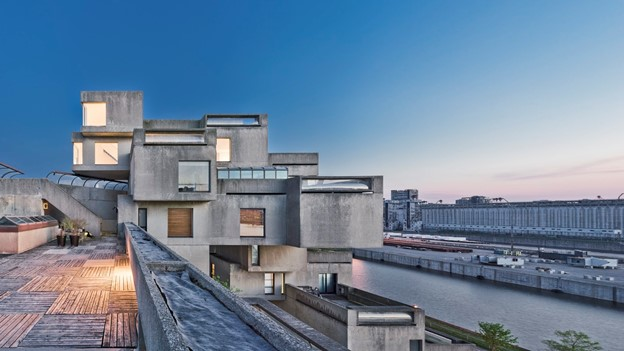
\includegraphics[height=\sampleimgh]{Figures/house.jpg}
        \label{fig:house_original}
      \end{tikzfigure}
    \end{minipage}
    \hfill
    \begin{minipage}[c]{0.475\linewidth}
      \begin{tikzfigure}[Vectorized image]
        \includesvg[height=\sampleimgh]{Figures/house.svg}
        \label{fig:house_svg}
      \end{tikzfigure}
    \end{minipage}

    \begin{minipage}[c]{0.475\linewidth}
      \begin{tikzfigure}[Original image]
        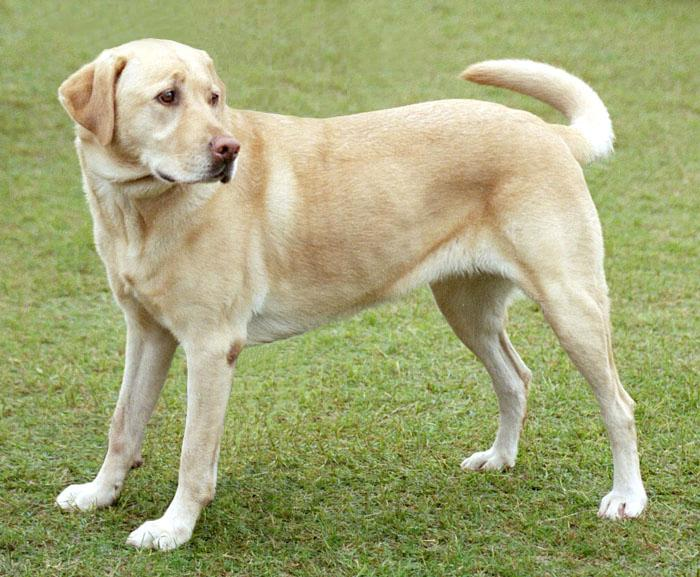
\includegraphics[height=\sampleimgh]{Figures/lab.jpg}
        \label{fig:lab_original}
      \end{tikzfigure}
    \end{minipage}
    \hfill
    \begin{minipage}[c]{0.475\linewidth}
      \begin{tikzfigure}[Vectorized image]
        \includesvg[height=\sampleimgh]{Figures/lab.svg}
        \label{fig:lab_svg}
      \end{tikzfigure}
    \end{minipage}
  }

  % TODO: describe the results briefly

  \column{0.05}

  \column{0.475}
  \block{Future Work}{
    {\fontsize{40}{48}\selectfont For the next iteration of our project, we need to combine our sampled points with the Potrace algorithm, which should improve the quality of edges on the final result. This will likely involve heuristic methods that directs mesh vectorization using the Potrace curves. The end goal is to improve the heuristics well enough to produce edges that resemble architectural line drawings.}
  }

  \block{References} {
    % \nocite{zhao2013image}
    % \nocite{dumoulin2017learned}
    % \nocite{hoppe1999new}
    % \nocite{selinger2003potrace}
    \printbibliography[
    heading=none
    ]

    % currently pointing to GitHub repo; later make it point to custom website
    % can we rename the repo to this
    \begin{flushright}
      \begin{minipage}[r]{128pt}
        \begin{tikzfigure}
          \includesvg[height=128pt]{qr-code.svg}
          \label{fig:qr-code}
        \end{tikzfigure}
      \end{minipage} \\
      \fontsize{16}{16}{\selectfont GitHub: Victoooooor/Vectorize-Arch}
    \end{flushright}
  }
\end{columns}


\end{document}
